\chapter{Planar Graphs}
Ajur was so enamored by Hamiltonian cycles, he was eager to meet Rishnak and hear more about them. Rishnak wanted to introduce a different concept: drawing graphs.
A planar drawing of a graph is one in which no edges cross each other (except at
the vertices). By definition, a \emph{planar graph} is a graph for which there exists at least one planar drawing.
If a graph does not admit any planar drawings, we call it a \emph{non-planar graph}.
For example here are two drawings of a complete graph on four vertices $K_4$. Since Figure \ref{9g2} has no edges crossing, we can call $K_4$ a planar graph.
\begin{figure}
\begin{center}
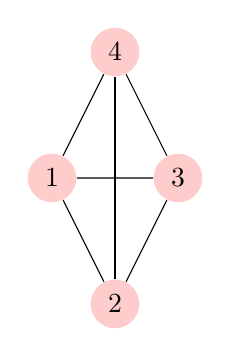
\begin{tikzpicture}
  [scale=.4,auto=left,every node/.style={circle,fill=red!20}]
  \node (n1) at (1,7) {1};
  \node (n2) at (3,3)  {2};
  \node (n3) at (5,7)  {3};
  \node (n4) at (3,11)  {4};

  \foreach \from/\to in {n1/n2,n2/n3,n2/n4,n1/n4,n3/n4,n1/n3} 
  \draw (\from) -- (\to);

\end{tikzpicture}
\caption{ Drawing of $K_4$ in which edges cross}\label{9g1}
\end{center}
\end{figure}
\begin{figure}
\begin{center}
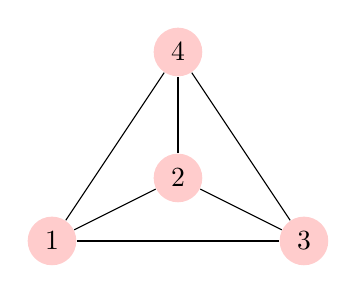
\begin{tikzpicture}
  [scale=.4,auto=left,every node/.style={circle,fill=red!20}]
  \node (n1) at (-1,7) {1};
  \node (n2) at (3,9)  {2};
  \node (n3) at (7,7)  {3};
  \node (n4) at (3,13)  {4};

  \foreach \from/\to in {n1/n2,n2/n3,n2/n4,n1/n4,n3/n4,n1/n3}
    \draw (\from) -- (\to);

\end{tikzpicture}
\caption{ Planar drawing of $K_4$}\label{9g2}
\end{center}
\end{figure}
 Rishnak asked Ajur whether he could draw the graph in Figure \ref{9g3} with no edges crossing.
 \begin{figure}
\begin{center}
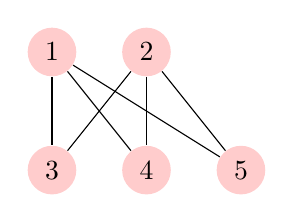
\begin{tikzpicture}
  [scale=.3,auto=left,every node/.style={circle,fill=red!20}]
  \node (n1) at (1,7) {1};
  \node (n2) at (5,7)  {2};
  \node (n3) at (1,2)  {3};
  \node (n4) at (5,2) {4};
  \node (n5) at (9,2)  {5};
 
  
   \foreach \from/\to in {n1/n3,n1/n4,n1/n5,n2/n3,n2/n4,n2/n5}
    \draw (\from) -- (\to);
    \end{tikzpicture}
\caption{ A bipartite graph with 5 vertices and 6 edges, denoted by $K_{2,3}$, where the edges cross}\label{9g3}
\end{center}
\end{figure}
Ajur thought for a while and found it a bit challenging. Then he thought of moving the vertex 2 down in which case no edges will cross. He drew the graph as shown in Figure \ref{9g4}
\begin{figure}
\begin{center}
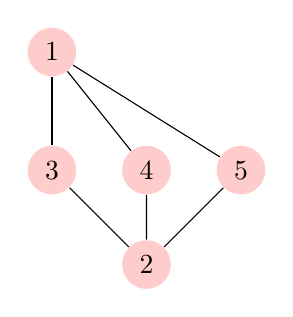
\begin{tikzpicture}
  [scale=.3,auto=left,every node/.style={circle,fill=red!20}]
  \node (n1) at (1,7) {1};
  \node (n2) at (5,-2)  {2};
  \node (n3) at (1,2)  {3};
  \node (n4) at (5,2) {4};
  \node (n5) at (9,2)  {5};
 
  
   \foreach \from/\to in {n1/n3,n1/n4,n1/n5,n2/n3,n2/n4,n2/n5}
    \draw (\from) -- (\to);
    \end{tikzpicture}
\caption{ Planar drawing of a bipartite graph $K_{2,3}$ with 5 vertices and 6 edges, with no edge crossings}\label{9g4}
\end{center}
\end{figure}

Impressed, Rishnak then asked Ajur whether the graph in Figure \ref{9g5} has a planar representation. Ajur struggled and tried to get a planar drawing --- but ended up with one edge crossing, see Figure \ref{9g6}. 

\begin{figure}
\begin{center}
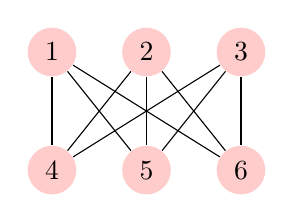
\begin{tikzpicture}
  [scale=.3,auto=left,every node/.style={circle,fill=red!20}]
  \node (n1) at (1,7) {1};
  \node (n2) at (5,7)  {2};
  \node (n3) at (9,7) {3};
  \node (n4) at (1,2)  {4};
  \node (n5) at (5,2) {5};
  \node (n6) at (9,2)  {6};
 
  
   \foreach \from/\to in {n1/n6,n1/n4,n1/n5,n2/n6,n2/n4,n2/n5,n3/n4,n3/n5,n3/n6}
    \draw (\from) -- (\to);
    \end{tikzpicture}
\caption{ A bipartite graph with 6 vertices and 9 edges, denoted by $K_{3,3}$, where the edges cross}\label{9g5}
\end{center}
\end{figure}
\begin{figure}
\begin{center}
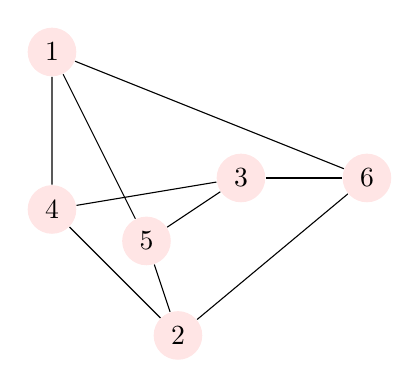
\begin{tikzpicture}
  [scale=.4,auto=left,every node/.style={circle,fill=red!10}]
  \node (n1) at (1,7) {1};
  \node (n2) at (5,-2)  {2};
  \node (n3) at (7,3) {3};
  \node (n4) at (1,2)  {4};
  \node (n5) at (4,1) {5};
  \node (n6) at (11,3)  {6};
 
  
   \foreach \from/\to in {n1/n6,n1/n4,n1/n5,n2/n6,n2/n4,n2/n5,n3/n4,n3/n5,n3/n6}
    \draw (\from) -- (\to);
    \end{tikzpicture}
\caption{ A  drawing of a bipartite graph with 6 vertices and 9 edges, denoted by $K_{3,3}$, where just two edges edges cross}\label{9g6}
\end{center}
\end{figure}
Rishnak then told Ajur that this graph does not have a planar representation. He added that there is a well-known related puzzle credited to Sam Loyd\footnote{Sam Loyd is a famous American recreational mathematician and puzzler.}. There are three houses (represented as circles) drawn on paper and below them three smaller circles representing gas, water, and electricity suppliers. The aim of the puzzle is to draw lines to get each utility into every house, without crossing over any line. Ajur reminded himself that he should read up on Loyd's puzzle books from his local library.

 Rishnak asked Ajur if two graphs $G$ and $H$ are isomorphic and if $G$ is planar, can you say $H$ is planar. Ajur said if $H$ is isomorphic to $G$, then each vertex corresponds to some vertex of $G$. By just relabeling the vertices of $G$ in its planar drawing, we get a planar drawing of $H$.
 
 Ajur then excitedly told Risnak that all trees have a planar representation\footnote{Ajur liked monkeys and monkeys liked trees. It followed by transitivity that Ajur liked trees.}. Rishnak answered that trees are indeed easy to embed in a plane as there are
 no cycles. He added that there are interesting space-filling planar representations of trees, for example in Figure \ref{9g7}.
\begin{figure}
\begin{center}    

 \begin{tikzpicture}[decoration=H-tree, very thick]
    \draw decorate { decorate { decorate { decorate { decorate { decorate { (0,0) -- (3,0) }}}}}};
  \end{tikzpicture}
  \caption{ A planar drawing of a tree (which is self similar)}\label{9g7}
  \end{center}
\end{figure}

One way to get a planar drawing is to embed the longest cycle in a plane and then try to place the rest of the vertices so that no edges cross each other. This cycle will divide the plane into two regions --- the inner region (inside the cycle) and the outer region (outside the cycle). So the edges have to go either inside or outside. By trying out the possibilities, you can get a planar representation of a graph (if one exists). Of course, this process is easier said than done. There is in fact an efficient method of placing the edges, without any backtracking, but Rishnak added that details are rather complicated. 

Each region in a planar representation is also referred to as a face. Euler discovered a remarkable formula concerning the number of edges, $e$, the number of vertices, $n$, and the number of faces, $f$ of a planar graph:
\begin{equation}
\label{eqn:euler}
  f-e+n=2 
\end{equation}

 

Rishnak proceeded to give an intuitive explanation of this formula \ref{eqn:euler}. Each region corresponds to a cycle and the external region (sometimes called an infinite region) also comes from a cycle. 
There are $n-1$ edges in a tree, and the rest of the $e-(n-1)$ edges in a graph will form part of a cycle. We will show in chapter 11. a spanning tree in a connected graph and how to choose one.
%\textbf{You implicitly pick a spanning tree, which you have not yet discussed! Consider saying: it turns out, as we'll learn in Chapter ***, that there exists a ``maximal tree" of any graph.} 
Each of these cycles correspond to an internal region or internal face, and there is one external face. From this, Euler's equation \ref{eqn:euler} follows.
\begin{eqnarray}
    \label{eqn:cycles}
    \text{internal faces}&=&e-(n-1)\nonumber\\
    \text{external face}&=&1 \nonumber \\
    \text{total faces}&=& \text{internal faces}~+~\text{external face} \nonumber \\
    &=&e-n+2
\end{eqnarray}

Ajur said that he has constructed Platonic solids with Zometools\footnote{Zometool is a commercial kit to make general polyhedra.}. Rishnak then explained Euler's equation applied for the five platonic solids; the graph theory in Euler's formula can be used to relate vertices, edges, and faces of the platonic solids! See Table \ref{tab:platonic} where $n$ stands for the number of vertices, $e$ stands for the number of edges and $f$ stands for the number of faces. All Platonic solids have a planar representation as shown in Figures \ref{fig:tetra}, \ref{fig:octa}, \ref{fig:cube}, \ref{fig:dod}, and \ref{fig:ico}\footnote{The reason is that every platonic solid embeds in sphere, and can be chosen such that no point or vertex passes the North pole. Then one may stereographically project the graph to the plane.}.
\begin{table}[ht]
    \centering
    \begin{tabular}{||c|c|c|c||}
    \hline
    Solid & n & e& f \\ [0.5ex] 
 \hline\hline
 Tetrahedron& 4 & 6 & 4 \\ 
 \hline
 Octohedron & 6 & 12& 8 \\
 \hline
 Cube & 8 & 12 & 6 \\
 \hline
 Dodecahedron & 20 & 30 & 12 \\
 \hline
 Icosahedron & 12 & 30 & 20 \\ [1ex] 
 \hline
 \end{tabular}
    \caption{Euler Equation for Platonic Solids}
    \label{tab:platonic}
\end{table}
\begin{figure}

  
\begin{tikzpicture}
[scale=0.7]
        \grTetrahedral
    \end{tikzpicture}
\caption{tetrahedron}
\label{fig:tetra}
\end{figure}
\begin{figure}
    \begin{tikzpicture}

        \grOctahedral[RA=5,RB=1]
    \end{tikzpicture}
\caption{Octahedron}\label{fig:octa}
\end{figure}
\begin{figure}
    \begin{tikzpicture}

        \grCubicalGraph
    \end{tikzpicture}
\caption{Cube}\label{fig:cube}
\end{figure}
\begin{figure}
    \begin{tikzpicture}
    [scale=0.8]

        \grDodecahedral[form=2] 
    \end{tikzpicture}
    \caption{Dodecahedron}\label{fig:dod}
\end{figure}
\begin{figure}
    \begin{tikzpicture}

        \grIcosahedral[form=2,RA=8]
    \end{tikzpicture}
\caption{Icosahedron}\label{fig:ico}
\end{figure}

Rishnak said each edge appears in exactly two faces. If each face is a triangle (cycle of length 3), it is called a maximal planar graph. Hence we deduce $e=\frac{3 \times f}{2}$ or $f=\frac{2 \times e}{3}$ . Substituting for $f$ in Euler's equation \ref{eqn:euler}, we get

\begin{eqnarray}
  \label{eqn:maxplanar}  
    \frac{2\times e}{3}&=&e-n+2\nonumber\\
    -\frac{e}{3} &=&-n+2\nonumber \\
    \frac{e}{3}&=&n-2 \nonumber \\
    e&=& 3 \times n - 6
\end{eqnarray}

Using Equation \ref{eqn:maxplanar}, it can be shown that the complete graph on 5 vertices, $K_5$ shown in Figure \ref{9g10}, is nonplanar. That graph has $n$=5, $e$=10. If it were planar then the number of edges would have to be at most $9$. 
Rishnak asked Ajur: can you use Euler's equation to show that $K_{3,3}$, a complete bipartite graph on 6 vertices (discussed in Figure \ref{9g5}), is nonplanar? 
Ajur was alert and he knew that the bipartite graph has only even cycle lengths. To have the maximum number of edges each face has to be of a cycle length 4. Hence $2\times e =4 \times f$ or $f=\frac{e}{2}$. Substituting for $f$ in Euler's equation \ref{eqn:euler}
$f=e-n+2$, one gets $-\frac{e}{2}=n-2$ or $e=2\times n -4$. Substituting for $n=6$, we get $e=8$. That is the maximum number possible. However, $K_{3,3}$ has 9 edges which is more than 8. Hence Ajur had proven that $K_{3,3}$ is nonplanar.
\begin{figure}
\begin{center}
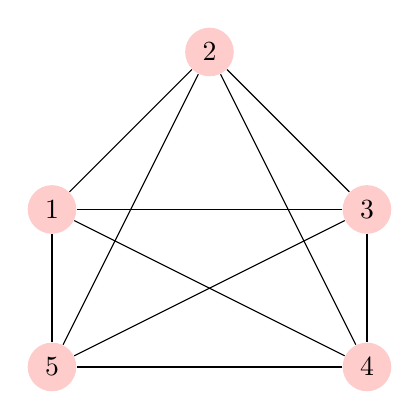
\begin{tikzpicture}
  [scale=.5,auto=left,every node/.style={circle,fill=red!20}]
  \node (n1) at (1,7) {1};
  \node (n2) at (5,11)  {2};
  \node (n3) at (9,7)  {3};
  \node (n4) at (9,3) {4};
  \node (n5) at (1,3) {5};

  \foreach \from/\to in {n1/n2,n2/n3,n3/n4,n4/n5,n1/n5,n1/n3,n1/n4,n2/n4,n2/n5,n3/n5}
    \draw (\from) -- (\to);

\end{tikzpicture}
\caption{ Complete Graph, $K_5$ with 5 vertices and 10 edges }\label{9g10}
\end{center}
\end{figure}
Rishnak added another interesting fact (without adding any further details) that any planar graph has not only a plane representation but also a representation in which each edge is drawn as a straight line.

Ajur responded that every subraph of a planar graph is also a planar graph. Pleased to note that Ajur was following the concepts, Rishnak added that the operation of dividing an edge, i.e., introducing vertices of degree 2 will not change the embedding. If a graph is planar and if we subdivide an edge, it is still planar. Similarly if a graph is nonplanar, and if e subdivides any edge, the graph is still nonplanar. An example of subdivision of an edge is shown in Figure \ref{9g9}. Now Jura appeared to be getting restless and Rishnak decided that they had had enough for that session, so they parted for the night.

\begin{figure}[h]
\begin{center}
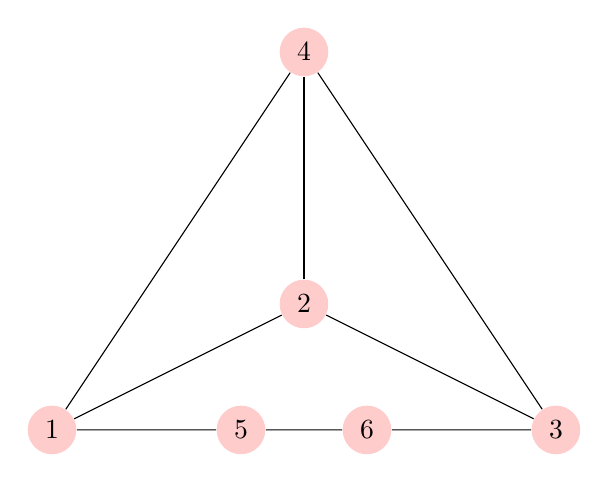
\begin{tikzpicture}
  [scale=.8,auto=left,every node/.style={circle,fill=red!20}]
  \node (n1) at (-1,7) {1};
  \node (n2) at (3,9)  {2};
  \node (n3) at (7,7)  {3};
  \node (n4) at (3,13)  {4};
  \node (n5) at (2,7) {5};
  \node (n6) at (4,7) {6};
 \foreach \from/\to in {n1/n2,n2/n3,n2/n4,n1/n4,n3/n4,n1/n5,n5/n6,n6/n3}
    \draw (\from) -- (\to);
\end{tikzpicture}
\caption{ Subdivision of edge (1,3) by adding two new vertices 5 and 6 in Figure \ref{9g2}}\label{9g9}
\end{center}
\end{figure}
